% arara: pdflatex: { synctex: yes }
% arara: makeindex: { style: ctuthesis }
% arara: bibtex

% The class takes all the key=value arguments that \ctusetup does,
% and a couple more: draft and oneside
\documentclass[twoside]{ctuthesis}

\ctusetup{
	preprint = \ctuverlog,
	mainlanguage = english,
	titlelanguage = english,
%	mainlanguage = czech,
	otherlanguages = {slovak,english},
	title-czech = {Moje bakalářka se strašně, ale hrozně dlouhým předlouhým názvem},
	title-english = {Drone detection using neural networks from combined RGB camera and LiDAR data},
	subtitle-czech = {Cesta do tajů kdovíčeho},
%	subtitle-english = {Journey to the who-knows-what wondeland},
	doctype = B,
	faculty = F3,
	department-czech = {Katedra matematiky},
	department-english = {Department of Cybernetics},
	author = {Adam Škuta},
	supervisor = {Matouš Vrba},
	supervisor-address = {Ústav X, \\ Uliční 5, \\ Praha 99},
	supervisor-specialist = {Martin Saska},
	fieldofstudy-english = {Mathematical Engineering},
	subfieldofstudy-english = {Mathematical Modelling},
	fieldofstudy-czech = {Matematcké inženýrství},
	subfieldofstudy-czech = {Matematické modelování},
	keywords-czech = {Dron, Konvolučná neurónová sieť, Detekcia, LiDAR, Riedky pointcloud},
	keywords-english = {Drone, Convolutional neural network, Detection, LiDAR, Sparse pointcloud},
	day = 10,
	month = 2,
	year = 2017,
	specification-file = {ctutest-zadani.pdf},
%	front-specification = true,
%	front-list-of-figures = false,
%	front-list-of-tables = false,
%	monochrome = true,
%	layout-short = true,
}

\ctuprocess

\addto\ctucaptionsczech{%
	\def\supervisorname{Vedoucí}%
	\def\subfieldofstudyname{Studijní program}%
}

\ctutemplateset{maketitle twocolumn default}{
	\begin{twocolumnfrontmatterpage}
		\ctutemplate{twocolumn.thanks}
		\ctutemplate{twocolumn.declaration}
		\ctutemplate{twocolumn.abstract.in.titlelanguage}
		\ctutemplate{twocolumn.abstract.in.secondlanguage}
		\ctutemplate{twocolumn.tableofcontents}
		\ctutemplate{twocolumn.listoffigures}
	\end{twocolumnfrontmatterpage}
}

% Theorem declarations, this is the reasonable default, anybody can do what they wish.
% If you prefer theorems in italics rather than slanted, use \theoremstyle{plainit}
\theoremstyle{plain}
\newtheorem{theorem}{Theorem}[chapter]
\newtheorem{corollary}[theorem]{Corollary}
\newtheorem{lemma}[theorem]{Lemma}
\newtheorem{proposition}[theorem]{Proposition}

\theoremstyle{definition}
\newtheorem{definition}[theorem]{Definition}
\newtheorem{example}[theorem]{Example}
\newtheorem{conjecture}[theorem]{Conjecture}

\theoremstyle{note}
\newtheorem*{remark*}{Remark}
\newtheorem{remark}[theorem]{Remark}

\setlength{\parskip}{5ex plus 0.2ex minus 0.2ex}
\graphicspath{{figures/}}

% Abstract in Czech
\begin{abstract-czech}
	Detekcia dron pomocou neurónových sietí z kombinovaných dát RGB kamery a LiDARu je popísaná v tejto práci. Viacero spôsobov kombinácie RGB kamery a LiDARu je prezentovaných. Samotná detekcia dron je realizovaná pomocou Konvolučnej neurónovej siete. Všetky metódy sú natrénované a otestované a následné výsledky sú porovnané s čistou RGB kamerou. Dáta používané v tejto práci boli vygenerované pomocou viacerých virtuálnych prostredí. Výsledky dokazujú, že v niektorých prípadoch RGBD metódy produkujú lepšie výsledky oproti RGB kamere v kontexte detekcie dronov. Budúca práca preto predstavuje ďaľšiu zaujímavú štúdiu.
\end{abstract-czech}

% Abstract in English
\begin{abstract-english}
The detection of drones using neural networks from combined RGB and LiDAR data is tackled in this thesis. Multiple approaches for RGB and LiDAR data fusion into RGBD data are presented. The detection of the drone is realized via a Convolutional neural network. All methods are trained and tested and the results are compared with the RGB only method. The dataset used in this thesis was generated using multiple Virtual environments. The results prove that there is a difference between RGBD and RGB approaches and in some specific scenarios RGBD approaches prove to be better than RGB ones in drone detection. Further work on these methods is, therefore, a worthwhile study.
\end{abstract-english}

% Acknowledgements / Podekovani
\begin{thanks}
Děkuji ČVUT, že mi je tak dobrou \emph{alma mater}.
\end{thanks}

% Declaration / Prohlaseni
\begin{declaration}
Prohlašuji, že jsem předloženou práci vypracoval samostatně, a že jsem uvedl veškerou použitou literaturu.

V Praze, \ctufield{day}.~\monthinlanguage{title}~\ctufield{year}
\end{declaration}

% Only for testing purposes
\listfiles
\usepackage[pagewise]{lineno}
\usepackage{lipsum,blindtext}
\usepackage{mathrsfs} % provides \mathscr used in the ridiculous examples
\usepackage{todonotes}
\usepackage{amsmath}
\usepackage{xspace}
\usepackage{caption}
\usepackage{subcaption}
\usepackage{multirow}
\usepackage{hyperref}
\usepackage{pdfpages}

\begin{document}

\maketitle
\chapter{Introduction}
In this thesis, drone detection using neural networks from combined RGB camera and LiDAR data is studied. With the recent development of drone technology, drones have become more readily available to the public and could only be expected to rise in popularity in the future. Drone detection is an important problem to tackle when it comes to tasks such as interception of uncooperative drones \cite{cite:1} or localization of drones in swarm \cite{cite:2} \cite{cite:3}. All methods presented in this thesis belong to the relative localization category. Compared to absolute localization methods, relative localization does not need to rely on pre-existing ground infrastructure and can be used in more environments. A Light detecting and ranging (LiDAR) sensor has been utilized on drones on multiple occasions \cite{cite:4} \cite{9553611} \cite{9554023} and RGB camera provides an easily accessible, cheap and lightweight sensor. Therefore a fusion of data retrieved from both sensors and its impact on the overall drone detection problem is an interesting problem to tackle. The results can be useful for occasions where a drone is already equipped with a LiDAR sensor. Or they can provide further clarification, whether the addition of LiDAR sensor into the drone detection problem provides any advantage.
\section{Related Work}
Solving the problem of drone detection has been tackled in different ways. They mostly differ from the sensors that are utilized or by placing markers on flying drones.
\begin{itemize}
	\item \textbf{Static Sensors} Current State of the art drone detection techniques utilizing static sensors such as Radars, Acoustic sensors or Wi-Fi rely on pre-existing infrastructure. In \cite{8337899} Radar technology faces multiple challenges when detecting smaller aircrafts such as drones, because of their size and altitude of their flight, but shows promising results. When it comes to accoustic sensors, sound of the drone can be a very good source of information but depends heavily on the ambient sound of its environment\cite{8337899}. In \cite{drone-det-wifi} drones are detected using Wi-FI packets that are sent between the drone and its user. This method relies on the fact that most commercially available drones utilize Wi-Fi packets when it comes to communication with the end user. Only presence of the drone in the vicinity can be achieved and not its exact location.
	\item \textbf{Marker based detection} Part of relative localization techniques utilizes a set of markers that are placed on a target drone. In \cite{holter2020relative} an observer drone utilizing a spherical camera with $360\deg$ Field-of-View detects and localizes drones equipped with markers. This system is applied in real-time and provides accurate localization within 4cm. Another approach is provided in \cite{8651535}, where ultra-violet emitters are equipped on a drone and serve as markers for the detection of the ultra-violet sensor. This approach proved to be successful in real-life situations. The downside of utilizing visual markers on target drones is that a hardware modification of the target drone is required. Therefore this approach is not applicable to all situations, especially when the target drone is not cooperating.
	\item \textbf{Convolutional neural networks} Due to its popularity and advancements, object detection convolutional neural networks have become a very popular technique for relative drone detection such as YOLOv3 \cite{redmon2018yolov3}, CenterNet \cite{zhou2019objects}, RetinaNet \cite{lin2018focal} and FasterRCNN \cite{ren2016faster}. One approach of using a convolutional neural network is described in \cite{ali2018yolo3d}. This approach is similar to the approach presented in this thesis in the sense that it fuses RGB and LiDAR data and use them as input into the modified YOLOv2 \cite{redmon2016yolo9000} convolutional neural network. This approach represents the LiDAR point cloud as a Birds-eye-view map and outputs 7 degrees of freedom for detected objects. Another approach described in \cite{8988144} uses a convolutional neural network for the use of relative micro aerial vehicle detection. This approach uses tiny-YOLO architecture \cite{redmon2016yolo9000} and estimates the distance of the detected vehicle from the size of its bounding box. The results prove to be applicable in real-world scenarios. For this thesis a YOLOv3 architecture is utilized, due to its speed and simplicity making it easier for utilization of LiDAR data.
\end{itemize}
\section{Problem Statement}
The goal of this thesis was to examine whether usage of LiDAR data coupled with RGB images from camera is useful for the localization of drones in contrast to the usage of image data alone. The LiDAR and RGB camera were mounted on top of the observer drone, which took pictures and point clouds of the target drone. All the measurements were taken inside a virtual environment, with a realistic drone and sensor simulation. The dataset was then processed and used as the input for training and testing a Convolutional neural network for the object detection as can be seen in \autoref{fig:intro}. The preprocessing was as follows:
\begin{itemize}
	\item coordinate transformation for the non-matching coordinate systems,
	\item projection of 3d points into a 2d image,
	\item utilizing different processing methods on sparse LiDAR point cloud to make it denser,
	\item fusing RGB images and LiDAR data into RGBD images.
\end{itemize}
The output metrics were then compared with the RGB trained convolutional neural network metrics.
\begin{figure}
	\centering
	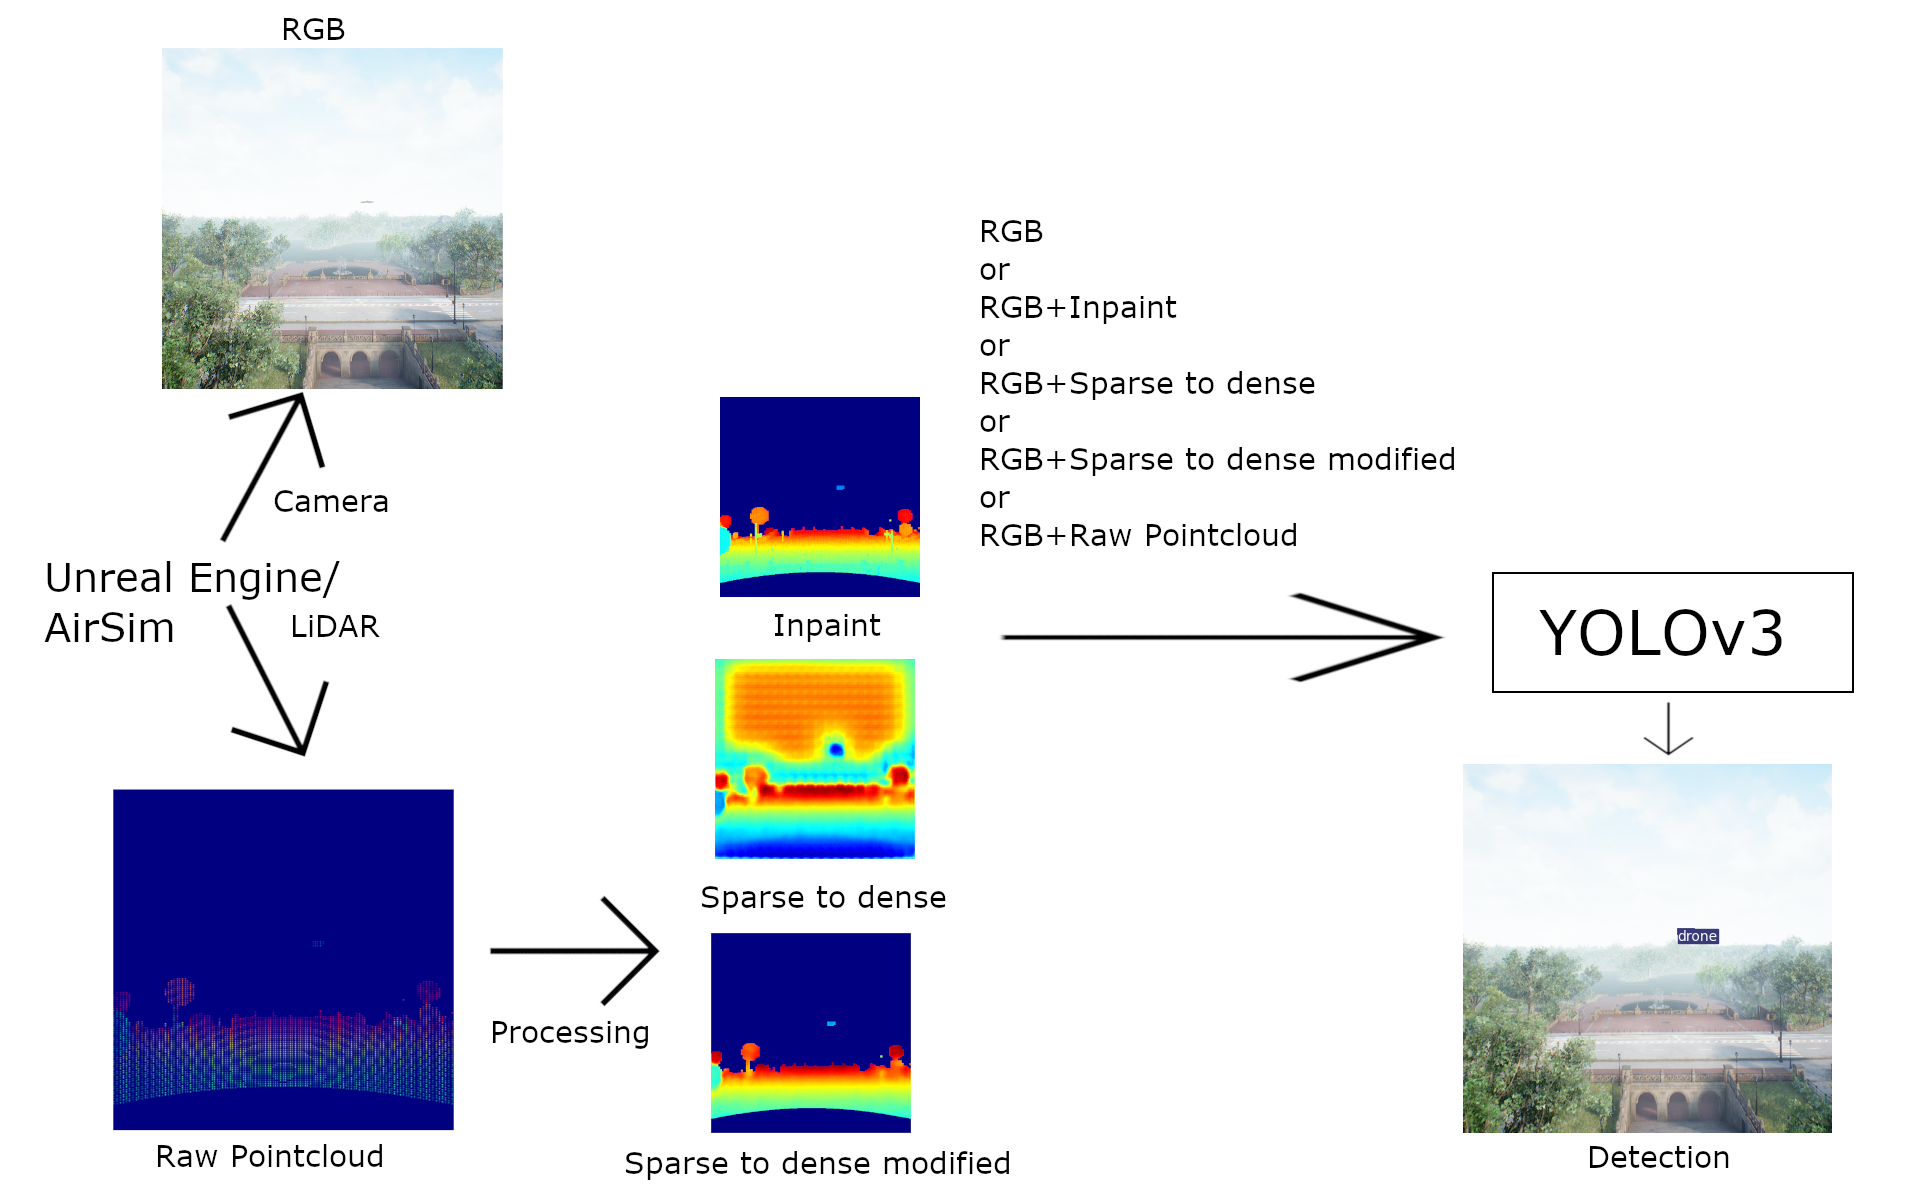
\includegraphics[width=\textwidth]{intro_schemav2.png}
	\caption{Schema of the process.}
	\label{fig:intro}
\end{figure}
\chapter{Methodology}
In this chapter, various methods used in this thesis are discussed. A video game engine Unreal Engine\footnote{\url{https://www.unrealengine.com}}paired with plugin AirSim\footnote{\url{https://microsoft.github.io/AirSim/}} was used for simulating real-life environments and for generating the dataset.\\
\\
One approach in this thesis was to input generated RGB data from the dataset and use it as an input into the YOLOv3 Convolutional neural network for drone detection.\\
\\
Another approach was to use Sparse to dense Convolutional neural network, which takes sparse LiDAR pointcloud and RGB image as an input and outputs dense LiDAR pointcloud. The neural network was pre-trained and its output was concatenated with RGB images and used as an input into the YOLOv3  for drone detection\\
\\
Another approach was to use the output of Sparse to dense network and further process the data, eliminating sections of the depth image that were very sparse and using the output concatenated with RGB images to use as input for YOLOv3.\\
\\
A separate approach was to use the inpainting method from the OpenCV Python library, which takes sparse LiDAR pointcloud and fills in unknown values based on the nearby known values, outputting dense pointcloud. The output of the inpainting method is further processed to filter inpainted values that were very far from known values and concatenated with RGB images to use as an input into YOLOv3.\\
\\
The final approach was to concatenate sparse LiDAR pointcloud with RGB images and use it as an input into YOLOv3.
\section{Sparse to dense} \label{s2d}
Sparse to dense is a Convolutional neural network written in PyTorch. \cite{ma2018sparsetodense} It predicts the depth measurements from a sparse depth dataset. The size of the network is modifiable and can be chosen as training parameters.
\begin{figure}
	\caption{Example of different network architectures available. Taken from \cite{ma2018sparsetodense}.}
	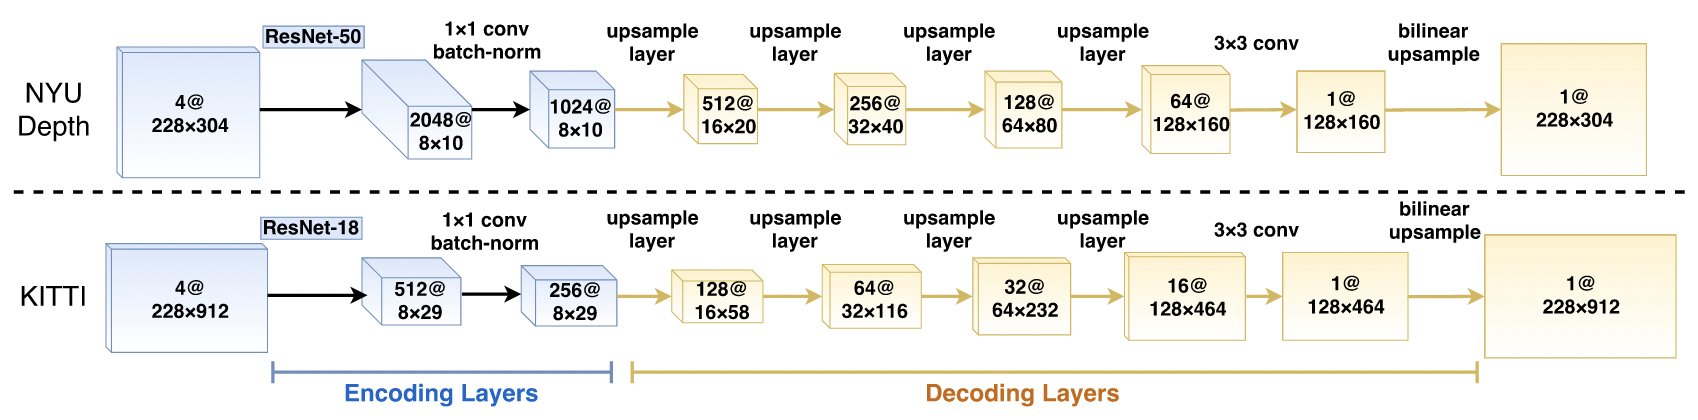
\includegraphics[width=\textwidth]{sparse2dense.png}
	\centering
	\label{fig:s2d_model}
\end{figure}
For the encoding and therefore input layers a ResNet-50 or ResNet-18 can be chosen, depending on the size of the input image for memory constraints as can be seen in \autoref{fig:s2d_model}. The decoding layers consist of 4 upsampling layers and a deconvolutional layer with either stride 2 or 3 or uprojection layer or upconvolutional layer as a choice for training. The default loss function is least absolute deviations also known as $L_1$ error:
\begin{equation}
	L_1=\sum_{i=1}^{n}|y_{true}-y_{predicted}|,
\end{equation}
where:
\begin{itemize}
	\item n is batch size,
	\item $y_{true}$ are real depth values,
	\item $y_{predicted}$ are predicted depth values.
\end{itemize}
The input to the network are RGBD images and the output is a depth map with the same dimensions as input. The depth input $D$ is sampled from the ground truth depth map $D^*$ with the following formula:
\begin{equation}
	D(i,j)=\begin{cases}
		D^*(i,j),&\text{with probability}\ p,\\
		0,&\text{otherwise},
	\end{cases}
\end{equation}
where:
\begin{itemize}
	\item $i,j$ are coordinates of the input image,
	\item $p=\frac{m}{n}$, where $m$ number of depth samples to be chosen at the start of training and $n$ is the total amount of available depth samples.
\end{itemize}
During training several input data augmentations take place. These augmentations include:
\begin{itemize}
	\item Scaling the input image by a random number $s\in[1,1.5]$,
	\item Rotating the input image by a random degree $r\in[-5,5]$,
	\item Scaling the brightness, contrast and saturation of the RGB component of the image by a random number $k\in[0.6,1.4]$,
	\item Normalizing the RGB component of the image,
	\item Flipping the image horizontally with a 50\% chance.
\end{itemize}
The output of the network is a dense depth image with the dimensions of the input. Every pixel contains predicted depth measurement in meters. The output of the Sparse to Dense network will be used for further training later.
\section{YOLOv3} \label{s:2.2}
You only look once (YOLO) is a convolutional neural network model used mainly for object detection and recognition\cite{redmon2016look}. The main advantage is its simplicity in comparison to similar convolutional neural networks, resulting in faster detection speeds. It belongs to the state of the art convolutional neural networks for object detection and recognition. The version used in this work is the third version YOLOv3\cite{redmon2018yolov3}. The backbone called Darknet53 consists of 53 convolutional layers. The original detector consists of 3 detection layers each responsible for detecting objects of various sizes as referred in \autoref{fig:yolov3_model}. 
\begin{figure}
	\caption{YOLOv3 network architecture. Taken from \cite{kathuria_2018}.}
	\centering
	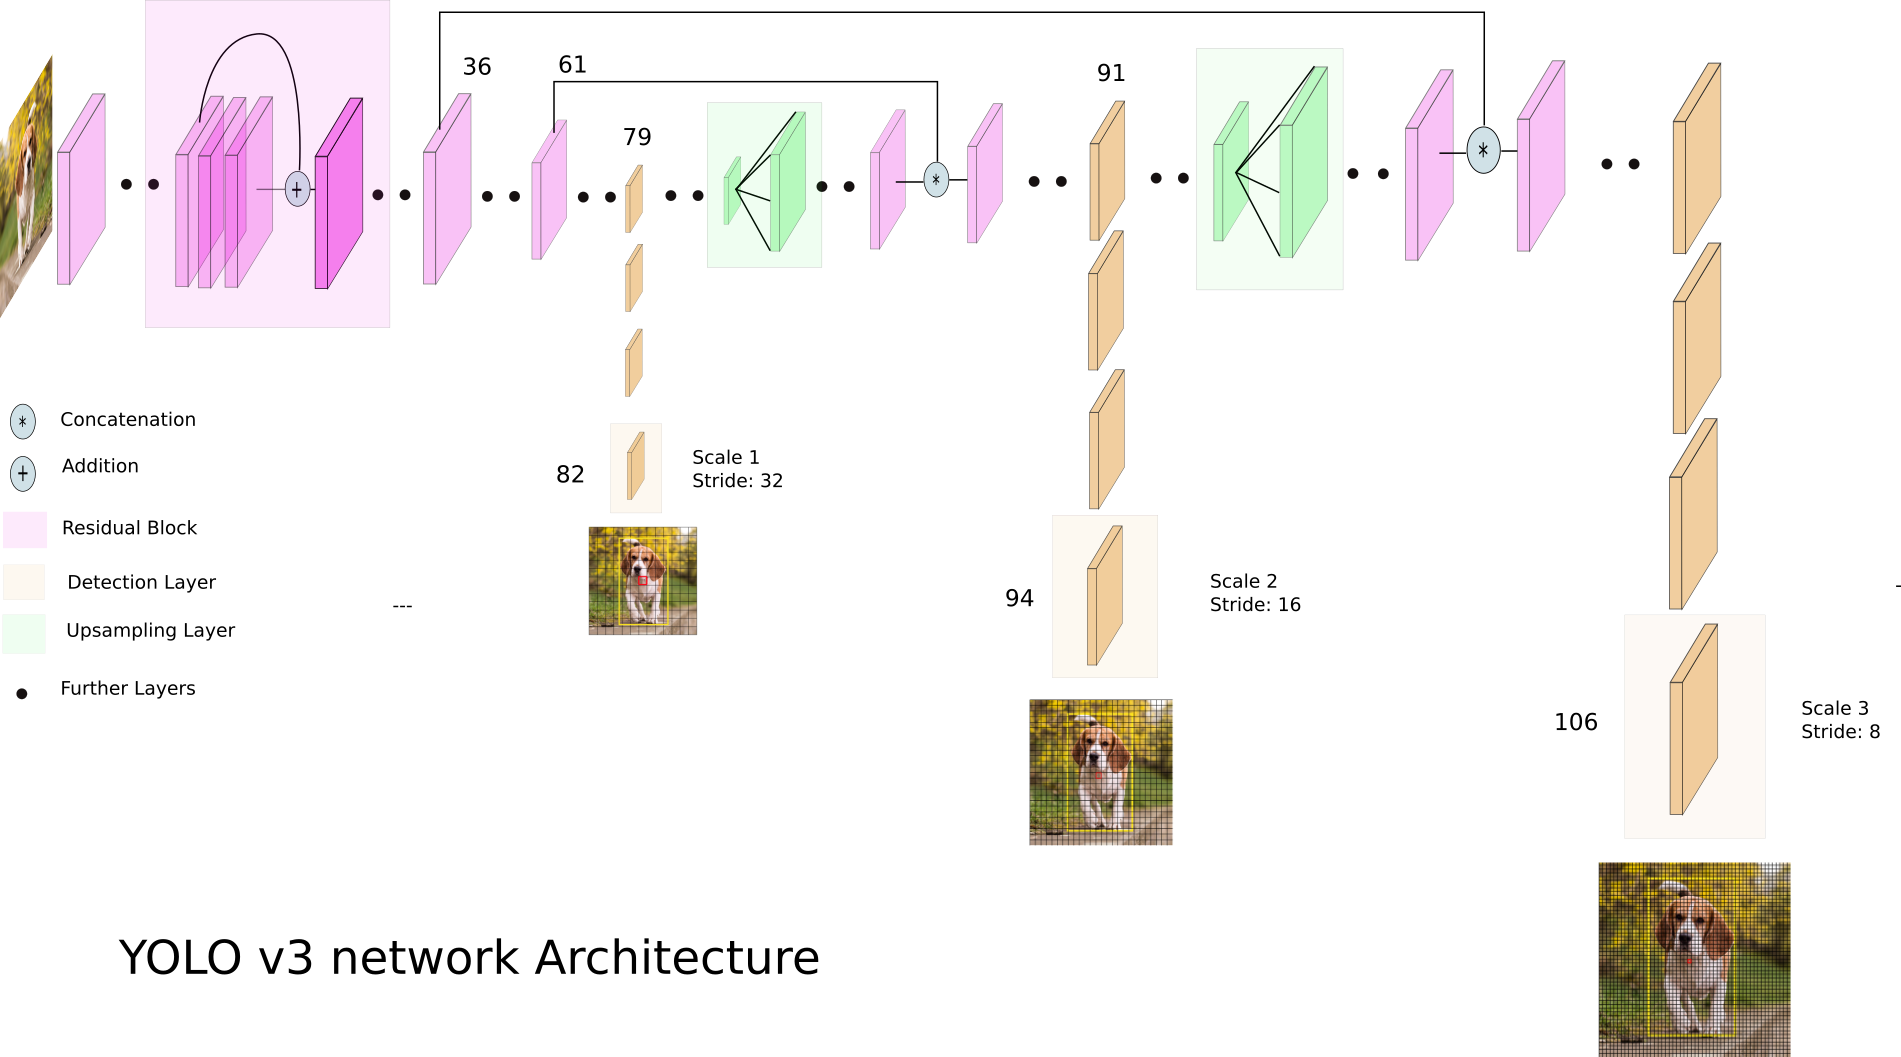
\includegraphics[width=\textwidth]{yolov3_model.png}
	\label{fig:yolov3_model}
\end{figure}
At each detection layer, the image is divided into multiple grid cells, where each grid cell detects three bounding boxes. YOLOv3 takes $n$-channel images as the input. Each of the detection layers outputs three bounding boxes for each of the cells. The content of one bounding box is as follows:
\begin{itemize}
	\item $t_x, t_y, t_w, t_h$ are bounding box co-ordinates,
	\item $p_O$ is objectness score,
	\item $p_c$ is class score for each class in the dataset.
\end{itemize}
The bounding box $t_x$ and $t_y$ coordinates are relative to the upper-left corner of its respective cell, while $t_w$ and $t_h$ are relative to one of the anchors. Anchors are pre-defined default bounding box sizes and can be modified before training. To transform these bounding box coordinates to be relative to the image following transformation is applied:
\begin{equation}\label{bbox}
	\begin{aligned}
		b_x&=\sigma(t_x)+c_x,\\
		b_y&=\sigma(t_y)+c_y,\\
		b_w&=p_{w}e^{t_w},\\
		b_h&=p_{w}e^{t_h},
	\end{aligned}
\end{equation}
where:
\begin{itemize}
	\item $\sigma(x)$ is a sigmoid function,
	\item $c_x, c_y$ are grid cells offsets from the top left corner of the image,
	\item $p_w, p_h$ are anchors width and height respectively,
	\item $b_x, b_y, b_w, b_h$ are bounding box coordinates relative to the image size.
\end{itemize}
The loss function used during the training is sum squared error loss or $L_2$ error described as follows:
\begin{equation}
	L_2=\sum_{i=1}^{n}(\mathbf{\hat{t}}-\mathbf{t})^2,
\end{equation}
where:
\begin{itemize}
	\item $n$ is batch size,
	\item $\mathbf{\hat{t}}$ is vector of predicted bounding box co-ordinates,
	\item $\mathbf{t}$ is vector of ground truth bounding box coordinates which can be obtained by inverting transformation in \ref{bbox}.
\end{itemize}
\section{Image inpainting method based on the Fast Marching Method} \label{inpainting}
Image inpainting is a method used for reconstructing missing values in the image. One such method based on \cite{cite:5} called the Image inpainting method based in the Fast Marching Method is presented in this section. A depth image is provided as the input. The same method can be extended for RGB images, but won't be needed for this thesis\\
\\
The depth value of a pixel to be inpainted is determined by the known neighbouring pixel values. To compute a depth value from one close pixel the following formula is used:
\begin{equation} \label{eq:1}
	I_q(\mathbf{p})=I(\mathbf{q})+\mathbf{\nabla I(q)}\cdot(\mathbf{p}-\mathbf{q}),
\end{equation}
where:
\begin{itemize}
	\item $\mathbf{q}$ is a vector of pixel coordinates with known depth value,
	\item $\mathbf{p}$ is a vector of pixel coordinates with unknown depth value,
	\item $I(x)$ is a depth value at pixel coordinates $\mathbf{x}$,
	\item $\mathbf{\nabla I(x)}$ is a gradient vector at pixel coordinates $\mathbf{x}$.
\end{itemize}
\begin{figure}[h]
	\centering
	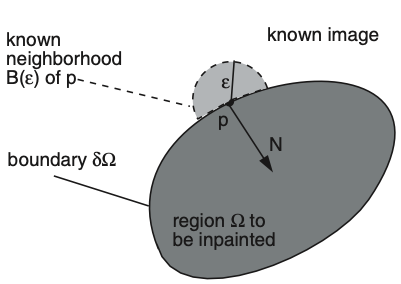
\includegraphics[width=9cm]{inpaint_principle.png}
	\caption{Inpainting principle. Image from: \cite{cite:5}}
	\label{fig:inpaint_schema}
\end{figure}
To get a final value for the unknown pixel the Equation \ref{eq:1} is applied on all known pixels in a specified region $B_{\varepsilon}(p)$ from the unknown pixel as can be seen in  \autoref{fig:inpaint_schema}. The function is as follows:
\begin{equation}\label{inpaint_eq}
	I(\mathbf{p})=\frac{\sum_{\mathbf{q}\in B_{\varepsilon}(\mathbf{p})}w(\mathbf{p},\mathbf{q})I_{\mathbf{q}}(\mathbf{p})}{\sum_{\mathbf{q}\in B_{\varepsilon}(\mathbf{p})}w(\mathbf{p},\mathbf{q})},
\end{equation}
where $w(\mathbf{p},\mathbf{q})$ is a weighting function designed for propagating sharpness of the image and is obtained as the product of the following equations:
\begin{equation}
	\begin{aligned}
		dir(\mathbf{p},\mathbf{q})&=\frac{\mathbf{p}-\mathbf{q}}{||\mathbf{p}-\mathbf{q}||}\cdot\mathbf{N(p)},\\
		dst(\mathbf{p},\mathbf{q})&=\frac{1}{||\mathbf{p}-\mathbf{q}||^2},\\
		lev(\mathbf{p},\mathbf{q})&=\frac{1}{1+|T(\mathbf{p})-T(\mathbf{q})|},
	\end{aligned}
\end{equation}
where,
\begin{itemize}
	\item $\mathbf{N(x)}$ is a normal vector of the boundary to be inpainted at pixel $\mathbf{x}$,
	\item $T(x)$ is distance of pixel $\mathbf{x}$ to the inpainting boundary.
\end{itemize}
The \eqref{inpaint_eq} is iteratively applied to all pixels on the inpainting boundary and advances inside the region to be inpainted until the whole region has been filled. This is implemented via the Fast Marching Method algorithm.
\begin{figure}
	\caption{Example of the inpainting technique. Image from: \cite{cite:5}.}
	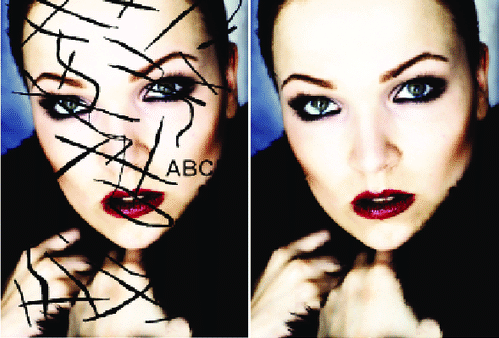
\includegraphics[width=10cm]{inpaint_example.png}
	\centering
\end{figure}
\section{Coordinate systems}
To correctly label the data for training, a position of the target drone in relation to the sensor mounted on the observer drone is required. The AirSim API returns the position of each drone in respect to their starting points. The starting point is a point where the drone spawns in the map. Therefore a transformation from the starting point of the target drone to the camera mounted on the observer is required. This transformation is written as follows:
\begin{equation}
	\textbf{T}=\textbf{T}_{o}^{c}\textbf{T}_{os}^{o}\textbf{T}_{ts}^{os},
\end{equation}
where:
\begin{itemize}
	\item $\textbf{T}_{ts}^{os}$ is transformation from the starting point of the target drone to the starting point of the observer drone,
	\item $\textbf{T}_{os}^{o}$ is transformation from the starting point of the  to the body of the first drone,
	\item $\textbf{T}_{o}^{c}$ is transformation from the body of the first drone to the cameras coordinate system.
\end{itemize}
\begin{figure}
	\centering
	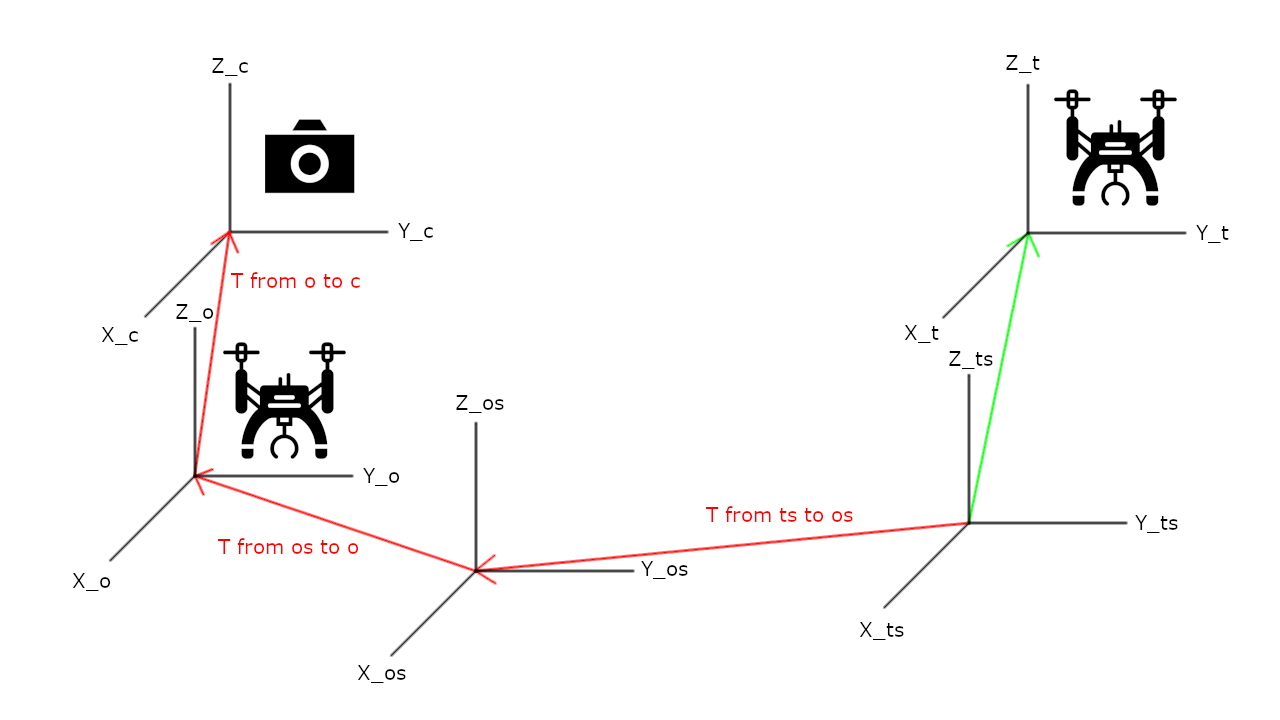
\includegraphics[width=\textwidth]{coord_schema.png}
	\caption{Visualization of transformation.}
	\label{fig:trans}
\end{figure}
Transformation matrix $\textbf{T}$ is generally be described as follows:
\begin{equation}
	\textbf{T}=\begin{bmatrix}
		\textbf{R} & \textbf{p}\\
		\textbf{0}^T & 1
	\end{bmatrix},
\end{equation}
where:
\begin{itemize}
	\item $\textbf{R}$ is a 3x3 rotation matrix,
	\item $\textbf{p}$ is a 3x1 translation column vector,
	\item $\textbf{0}^T$ is a 1x3 row vector of zeros.
\end{itemize}
To transform a location of the drone represented by vector $\mathbf{v_{ts}}$ into the coordinate system of the camera, as can be seen in \autoref{fig:trans}, the following transformation is applied:
\begin{equation}
	\mathbf{v_c}=\mathbf{T}\mathbf{v_{ts}}
\end{equation}
\section{Camera Model} \label{sec:camera-model}
For the creation of the bounding boxes used for training and for processing raw data from LiDAR sensor a transformation from coordinate system of the camera to the pixel values of the image needs to be defined. For this task a pinhole camera model is used.
\begin{figure}
	\centering
	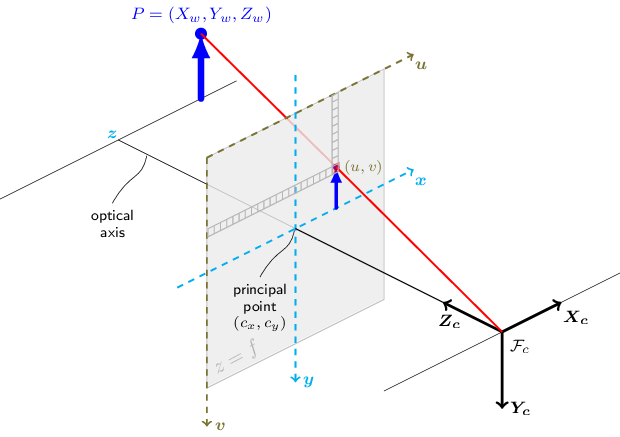
\includegraphics[width=\textwidth]{pinhole_camera_model.png}
	\caption{Pinhole camera model. Image from \cite{opencv}.}
\end{figure}\\
The transformation is then defined as follows:
\begin{equation} \label{eq:2}
	\begin{bmatrix}
		u\\
		v
	\end{bmatrix}=
	\begin{bmatrix}
		f\frac{X_c}{Z_c}+c_x\\
		f\frac{Y_c}{Z_c}+c_y
	\end{bmatrix},
\end{equation}
where:
\begin{itemize}
	\item $u$ and $v$ are pixel coordinate values on the image,
	\item $X_c$,$Y_c$,$Z_c$ are coordinate values of a point in the coordinate system of the camera,
	\item $f$ is focal length of the camera,
	\item $c_x$,$c_y$ are offsets on the image plane.
\end{itemize}
Pinhole camera model is only idealization of a real life camera and no lens distortion needs to be considered. The AirSim simulator simulates pinhole camera so no other processing needs to be done.
\section{Dataset} \label{s:2.6}
The dataset for this work can be generated in two ways. The first is real-life drone shots mixed with point clouds from LiDAR mounted on top of a drone. The second is generating a dataset using a realistic virtual environment where a drone, camera and LiDAR are being emulated very close to their real-life counterparts. An advantage to this approach is that a great variety of environments can be chosen a lot of them often inaccessible otherwise (power plant, airport, snowy mountains out of season etc.). Therefore this approach was chosen for the task.
\subsection{Unreal Engine}
Unreal Engine is a software tool used for creating realistic 3d environments, most often used as a video game engine. It is written in C++ and open-source supporting a variety of pre-built environments and assets. For this work three different environments were used for the creation of the dataset:
\begin{itemize}
	\item City Park Environment Collection (2256 samples taken),
	\item Automotive Winter Scene (1813 samples taken),
	\item Downtown West Modular Pack(1120 samples taken).
\end{itemize}
\begin{figure}
	\centering
	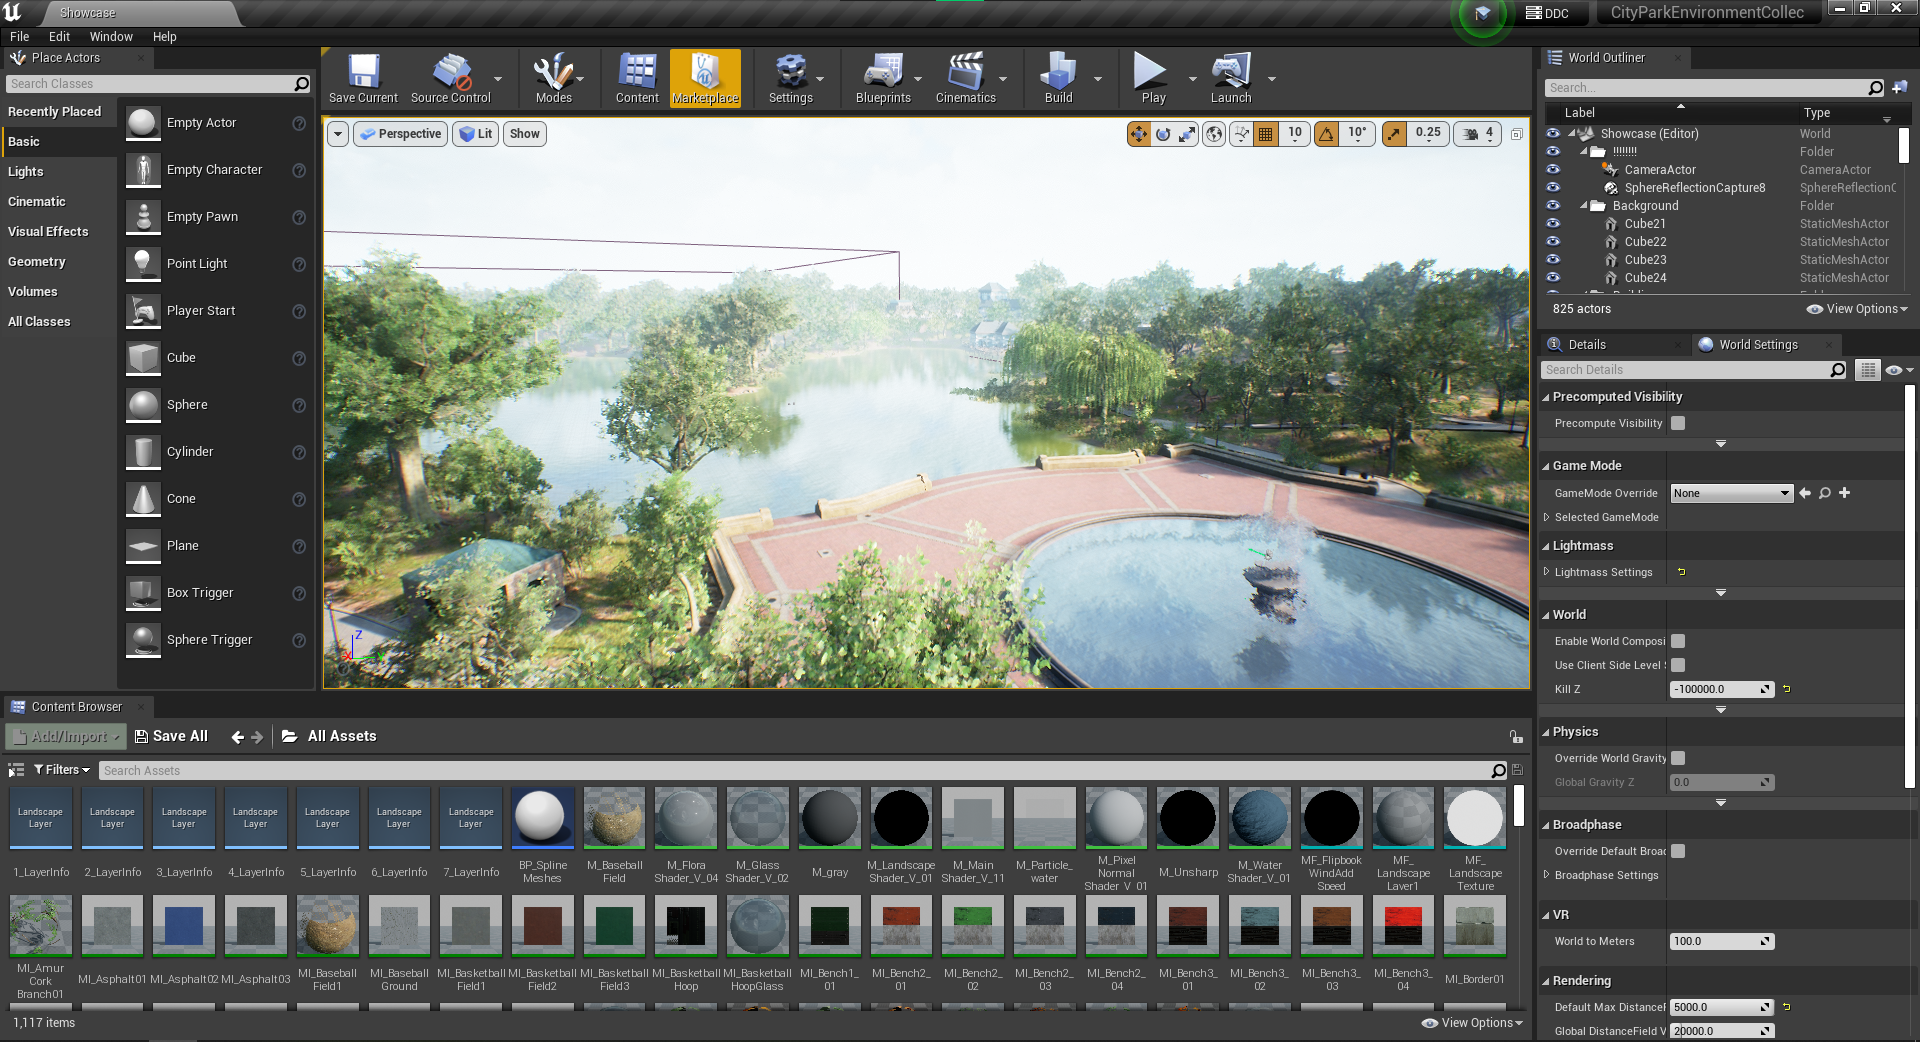
\includegraphics[width=\textwidth]{unreal_ui.png}
	\caption{Unreal Engine user interface.}
\end{figure}
Together 5320 pictures and labels were generated using two drones. The observer drone was equipped with an RGB camera and LiDAR sensor and was responsible for taking the pictures and pointclouds from LiDAR. The Parrot AR.Drone 2.0 shown in \autoref{fig:parrot} was used as a model for drone detection.
\begin{figure}
	\centering
	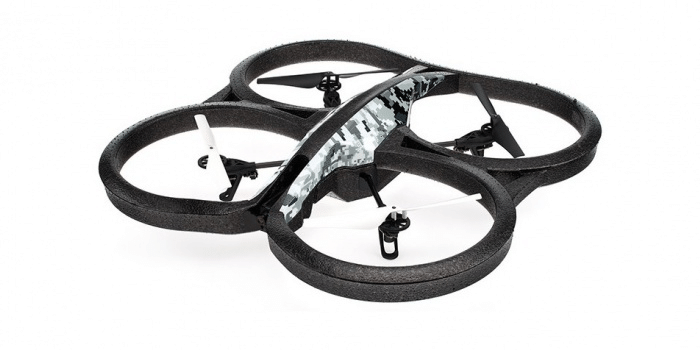
\includegraphics[width=\textwidth]{parrot.png}
	\caption{Parrot AR.Drone 2.0. Image taken from \cite{parrot}.}
	\label{fig:parrot}
\end{figure}
\subsection{AirSim}
An open-source plugin for Unreal Engine called AirSim was used for the generation of the dataset. It simulates realistic flight motions of drones as well as seven types of sensors, including RGB camera and LiDAR used for this task. AirSim supports both a C++ API as well as Python API, the latter of which was used for controlling the motion and capturing the dataset. The location of the second drone was generated through API call, which produces a location of the drone in local coordinates relative to its starting point, which is later transformed to the local coordinates of the first drone carrying the LiDAR and RGB sensors using \eqref{eq:2}. The bounding box required for the Convolutional neural network was generated the same way but the edge points of the 3D bounding box were transformed using \eqref{eq:2}. The bounding box dimensions were set to $(0.6, 1.0, 0.3)$. The LiDAR pointcloud was generated via an API call, which returned 3D pointcloud in relation to the observer drone. Therefore transformation \eqref{eq:2} was utilized. The capturing drone travelled on each map on a 3D cube grid.
\begin{figure}
	\centering
	\begin{subfigure}[b]{0.3\textwidth}
		\centering
		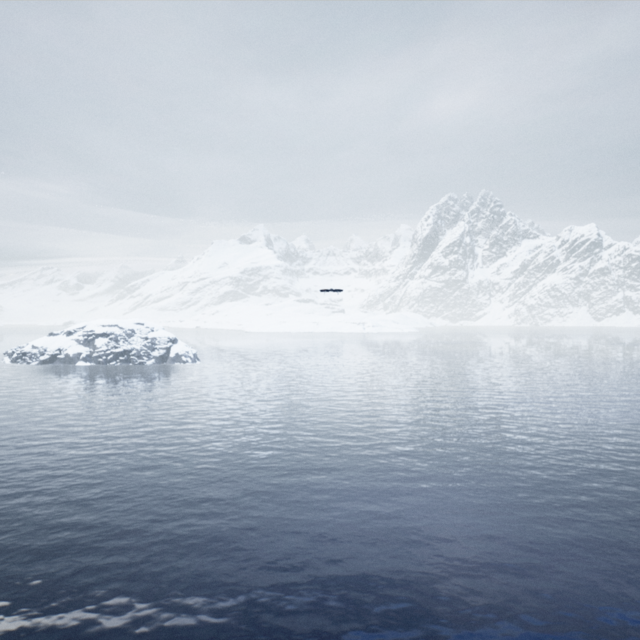
\includegraphics[width=\textwidth]{snow_rgb.png}
		\caption{Snow Environment.}
	\end{subfigure}
	\hfill
	\begin{subfigure}[b]{0.3\textwidth}
		\centering
		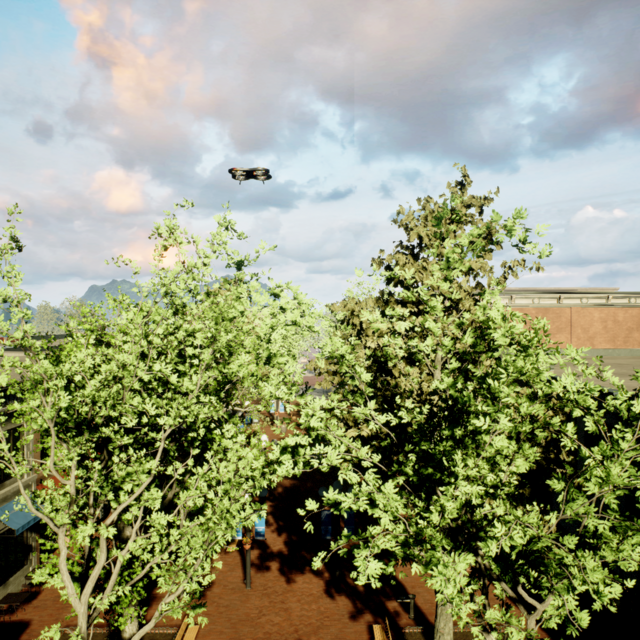
\includegraphics[width=\textwidth]{city_rgb.png}
		\caption{City Environment.}
	\end{subfigure}
	\hfill
	\begin{subfigure}[b]{0.3\textwidth}
		\centering
		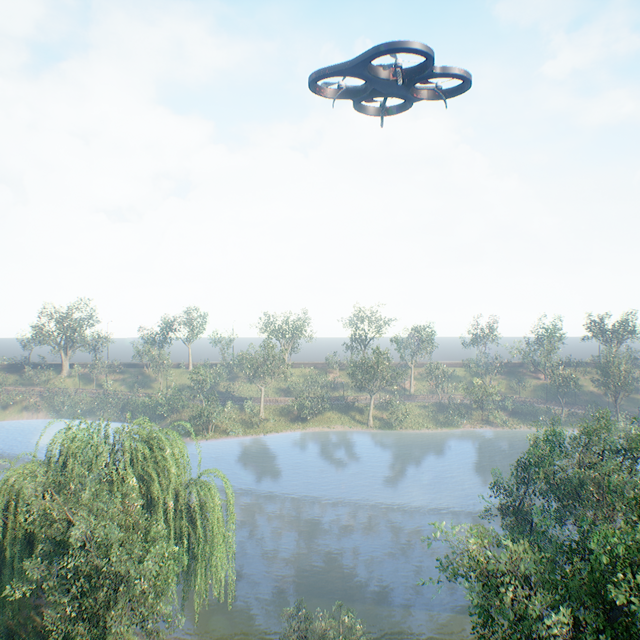
\includegraphics[width=\textwidth]{park_rgb.png}
		\caption{Park Environment.}
	\end{subfigure}
	\caption{Sample photos from each environment.}
\end{figure}
\section{Training}
For training purposes, 5320 samples were taken using the AirSim simulator. Each sample consists of:
\begin{itemize}
	\item 640x640 RGB image from the camera,
	\item 640x640 sparse depth image from the LiDAR sensor,
	\item Label file containing ground truth bounding boxes co-ordinates.
\end{itemize}
This dataset was split into 3662 training, 407 validation, 1251 testing samples.
\subsection{Sparse to Dense}
The data were trained using Sparse to Dense neural network to receive dense depth images. The training was done for 15 epochs using a batch size of 8. The backbone was Resnet18 and the decoder was set to Deconv3 as described in \autoref{s2d}. The network was trained on Kitti\footnote{\url{http://www.cvlibs.net/datasets/kitti/}} dataset.
\begin{figure}
	\centering
	\begin{subfigure}[b]{0.4\textwidth}
		\centering
		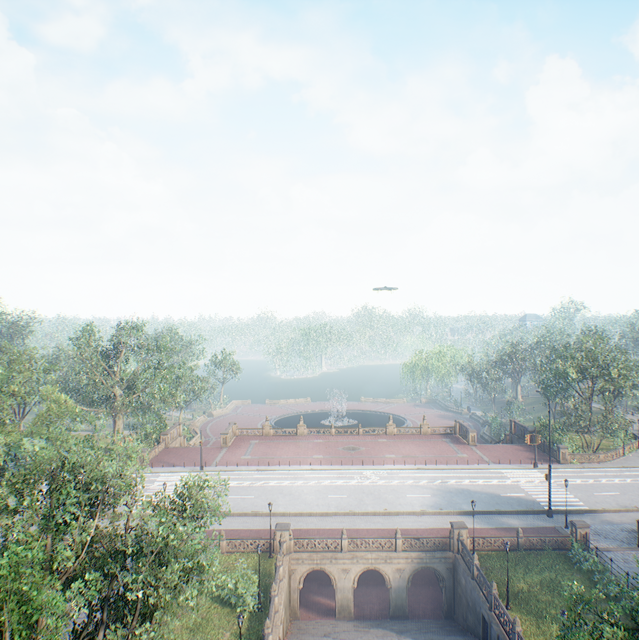
\includegraphics[width=\textwidth]{s2d_input.png}
		\caption{Input image.}
	\end{subfigure}
	\hfill
	\begin{subfigure}[b]{0.4\textwidth}
		\centering
		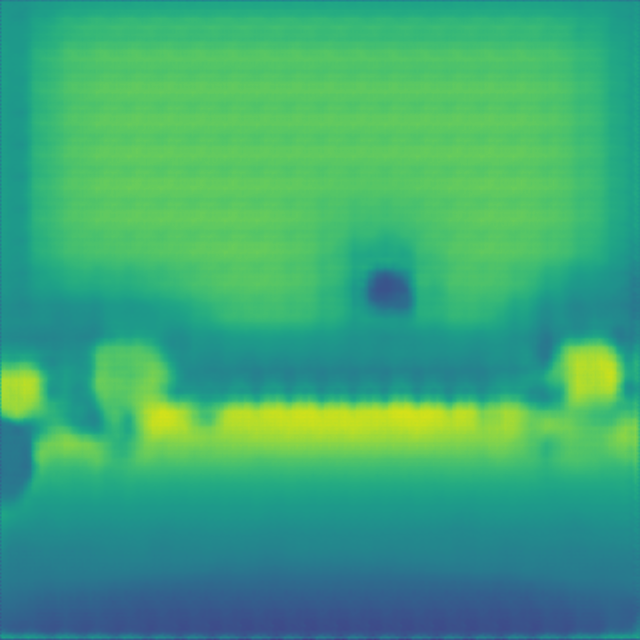
\includegraphics[width=\textwidth]{s2d_output.png}
		\caption{Output depth map.}
	\end{subfigure}
	\hfill
	\begin{subfigure}[b]{0.4\textwidth}
		\centering
		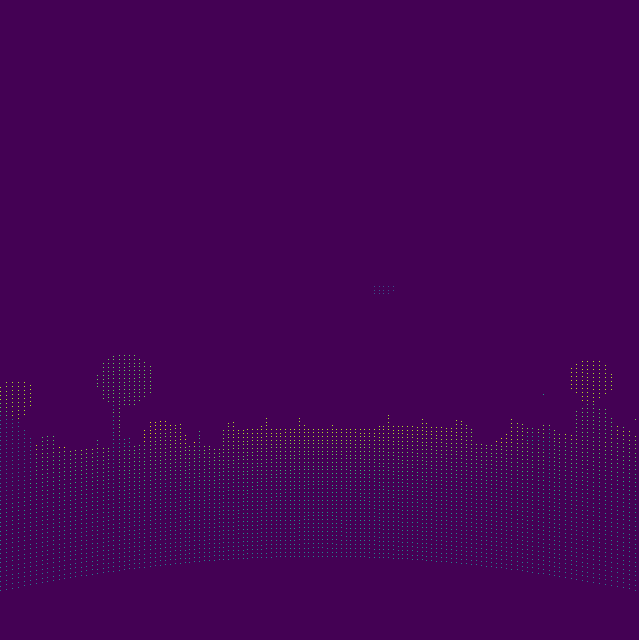
\includegraphics[width=\textwidth]{s2d_all.png}
		\caption{All pointcloud points.}
	\end{subfigure}
	\hfill
	\begin{subfigure}[b]{0.4\textwidth}
		\centering
		
\includegraphics[width=\textwidth]{s2d_select.png}
		\caption{Selected pointcloud points.}
	\end{subfigure}
	\caption{Sparse to dense training.}
	\label{fig:s2d_tr}
\end{figure}
A processing algorithm was applied to the output depth map, further filtering points that were not in the vicinity of the ground truth depth points. Both filtered and unfiltered depth maps were used for further training and testing to clarify their overall impact and the results can be seen in \autoref{fig:s2d_tr} and \autoref{fig:s2d_mod}.
\begin{figure}
	\centering
	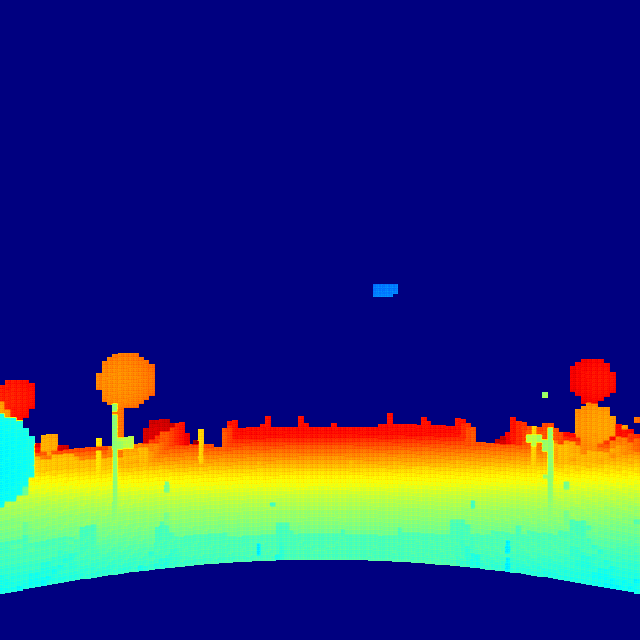
\includegraphics[width=5cm]{sparse2dense_filter.png}
	\caption{Applied filter on Sparse to dense output.}
	\label{fig:s2d_mod}
\end{figure}
\subsection{Image inpainting}
An alternative algorithm for making sparse pointcloud into dense ones was applied as well. The function is provided in the OpenCV Python library. The input into the function was a sparse depth image, same as for the Sparse to dense network except for the RGB part. The algorithm introduced in \ref{inpainting} was used with the radius of 1 pixel. The results were processed with the same filtering method as for the results of Sparse to dense method. For further training, only the filtered depth map was used.
\begin{figure}
	\centering
	\begin{subfigure}[b]{0.3\textwidth}
		\centering
		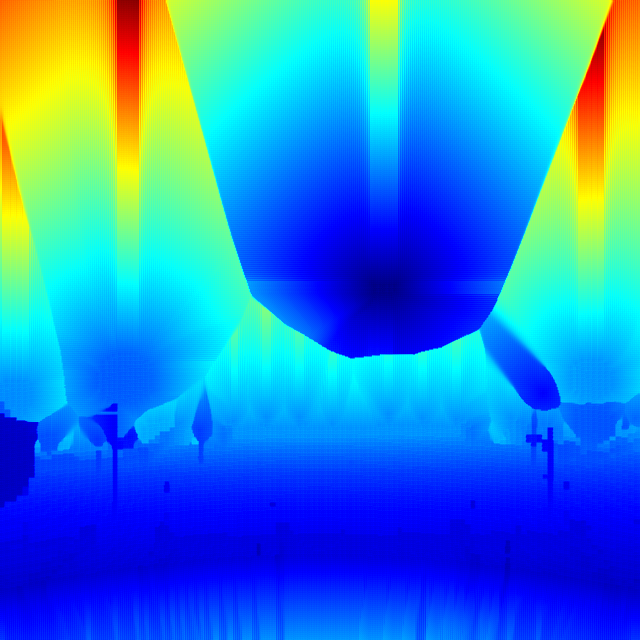
\includegraphics[width=\textwidth]{raw_inpaint.png}
		\caption{Non filtered result.}
	\end{subfigure}
	\hfill
	\begin{subfigure}[b]{0.3\textwidth}
		\centering
		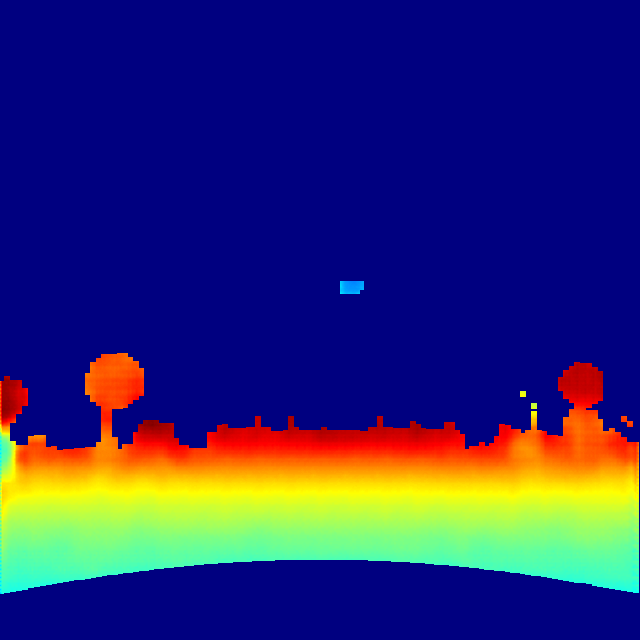
\includegraphics[width=\textwidth]{inpaint.png}
		\caption{Filtered result.}
	\end{subfigure}
	\caption{Inpaint results.}
\end{figure}
\subsection{YOLOv3}
The following parameters were used for training all inputs:
\begin{itemize}
	\item number of epochs was set to 120,
	\item batch size was set to 128,
	\item size of the input images was 416x416x$n$, where $n\in\{3,4\}$,
	\item learning rate was set to 0.001.
\end{itemize}
YOLOv3 PyTorch implementation was used for training\footnote{\url{https://github.com/eriklindernoren/PyTorch-YOLOv3}}. Further modifications were required to be made. The original implementation of YOLOv3 supports 3-channel RGB images as inputs. For the sake of this work an RGBD input option using the H5 file system was implemented. The dataset consisted of drones of various sizes ranging from very small (few pixels) to very large closeups. Therefore 5 detection heads were implemented instead of the original 3. This ensured much higher detection confidence of smaller far away drones as well as bigger more close ones.
\begin{figure}
	\centering
	\begin{subfigure}[b]{0.4\textwidth}
		\centering
		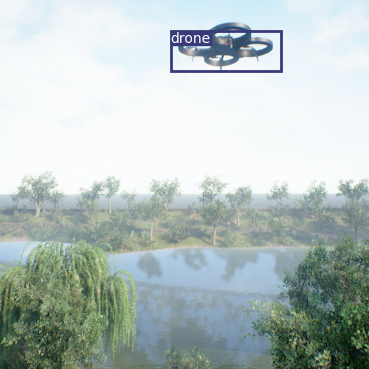
\includegraphics[width=\textwidth]{02167.png}
	\end{subfigure}
	\hfill
	\begin{subfigure}[b]{0.4\textwidth}
		\centering
		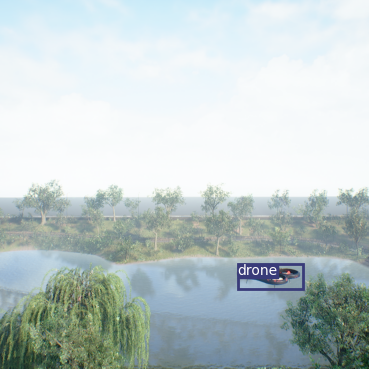
\includegraphics[width=\textwidth]{02665.png}
	\end{subfigure}
	\caption{Sample YOLOv3 outputs.}
\end{figure}
\chapter{Results}
After the training was completed the different metrics on the validation dataset were compared. These metrics include:
\begin{itemize}
	\item precision,
	\item recall,
	\item intersection over Union,
	\item mean Average Precision (mAP).
\end{itemize}
These metrics are given by the following formulas:
\begin{equation}
\begin{aligned}
	Precision &= \frac{\text{True Positives}}{\text{True Positives} + \text{False Positives}},\\
	Recall &= \frac{\text{True Positives}}{\text{True Positives} + \text{False Negatives}},\\
	IoU &= \frac{\text{Area of overlap of two bounding boxes}}{\text{Area of union of two bounding boxes}},\\
	mAP &= \frac{1}{N}\sum^N_{i=1}AP_i.
\end{aligned}
\end{equation}
where:
\begin{itemize}
	\item $N$ is number of classes,
	\item $AP$ is Average Precision, an area under the Precision Recall curve.
\end{itemize}
In this case, the dataset consisted of only one class, which is a drone. Therefore $mAP=AP$.
\begin{figure}
	\centering
	\begin{subfigure}[b]{0.49\textwidth}
		\centering
		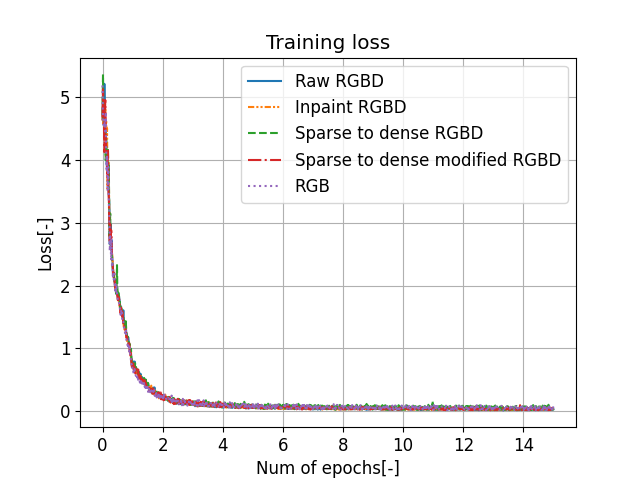
\includegraphics[width=\textwidth]{train_loss.png}
	\end{subfigure}
	\hfill
	\begin{subfigure}[b]{0.49\textwidth}
		\centering
		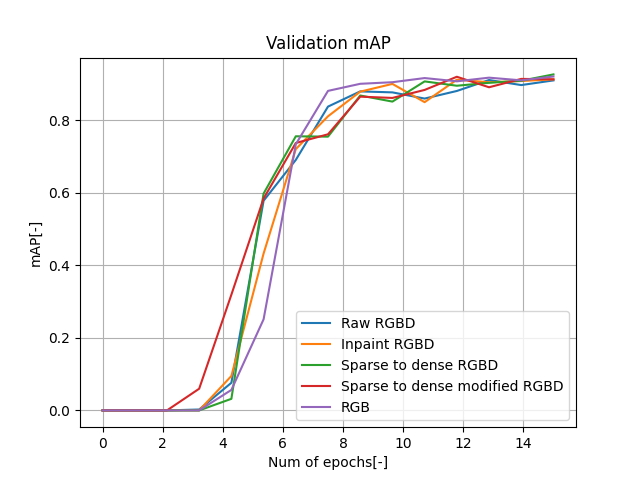
\includegraphics[width=\textwidth]{validation_mAP.png}
	\end{subfigure}
	\caption{Training results}
\end{figure}
For the training results validation mAP followed the training loss and started converging after around the 8th epoch. It fully stopped rising after the 12th epoch. Considering this the chosen weights ensured that the network does not overfit the training and validating dataset. \autoref{table:weights} shows selected weights for each method.
\begin{table}
	\begin{tabular}{|c|c|c|c|c|c|}
		\hline
		& \begin{tabular}[c]{@{}c@{}}Raw\\ RGBD\end{tabular} & \begin{tabular}[c]{@{}c@{}}Inpaint\\ RGBD\end{tabular} & \begin{tabular}[c]{@{}c@{}}Sparse to dense\\ RGBD\end{tabular} & \begin{tabular}[c]{@{}c@{}}Sparse to dense\\ modified RGBD\end{tabular} & RGB \\ \hline
		Weigths{[}epoch{]} & 9                                                  & 9                                                      & 11                                                             & 12                                                                      & 8   \\ \hline
	\end{tabular}
	\caption{Chosen weights.}
	\label{table:weights}
\end{table}\\
After the weights were chosen the network was validated on the test dataset. The confidence threshold was chosen to be $0.2$. The results were as follows:
\begin{table}[h]
	\begin{tabular}{|c|c|c|c|c|c|}
		\hline
		Results   & \begin{tabular}[c]{@{}c@{}}Raw\\ RGBD\end{tabular} & \begin{tabular}[c]{@{}c@{}}Inpaint\\ RGBD\end{tabular} & \begin{tabular}[c]{@{}c@{}}Sparse to dense\\ RGBD\end{tabular} & \begin{tabular}[c]{@{}c@{}}Sparse to dense\\ modified RGBD\end{tabular} & RGB  \\ \hline
		mAP       & \textbf{0.48}                                      & 0.46                                                   & 0.36                                                           & 0.43                                                                    & 0.41 \\ \hline
		Precision & 0.59                                               & 0.89                                                   & \textbf{0.92}                                                  & 0.60                                                                    & 0.79 \\ \hline
		Recall    & \textbf{0.53}                                      & 0.48                                                   & 0.37                                                           & 0.48                                                                    & 0.48 \\ \hline
		IoU       & 0.79                                               & \textbf{0.84}                                          & \textbf{0.84}                                                  & 0.83                                                                    & 0.83 \\ \hline
	\end{tabular}
	\caption{Testing results}
\end{table}\\
\pagebreak
\begin{figure}
	\centering
	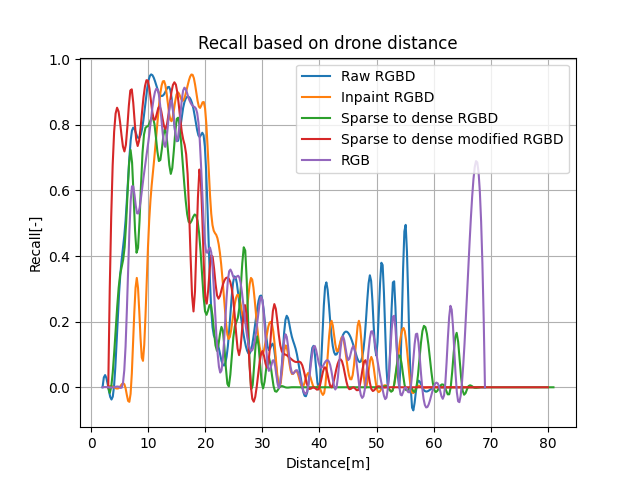
\includegraphics[width=\textwidth]{recall_distance.png}
	\caption{Recall based on distance of the drone.} \label{fig:recall_distance}
\end{figure}\\
From the results, Raw RGBD offers the best improvement in terms of mAP by 7\%. Every method except unmodified Sparse to dense offers some improvement in terms of mAP. In terms of precision unmodified Sparse to dense and Inpaint offer improvement over RGB by 13\% and 10\% respectively. Other methods namely Raw RGBD and modified Sparse to dense offer a decrease of 20\% and 19\% respectively. When it comes to recall not a big improvement is made. The best method is Raw RGBD with an increase of 5\% in comparison to RGB. Unmodified Sparse to dense suffers a decrease of 11\% in comparison to RGB, while the remaining methods are unchanged. This can be observed in \autoref{fig:recall_distance} where all methods perform the best in the range from 4 to 19 meters reaching a maximum recall of around 0.95. Modified Sparse to dense offers the highest recall in around 4 meters but starts to fall after 18 meters. Raw RGBD shows a few spikes in the range from around 48 to 55 meters, the highest reaching 0.5 recall. RGB shows a spike at around 67 meters with recall of around 0.7. In terms of IoU, all methods perform very similarly with best-performing methods Inpaint RGBD and unmodified Sparse to dense showing improvement of 1\%.
\pagebreak
\begin{table}[h]
	\begin{tabular}{|c|c|c|c|c|c|}
		\hline
		Speed       & \begin{tabular}[c]{@{}c@{}}Raw\\ RGBD\end{tabular} & \begin{tabular}[c]{@{}c@{}}Inpaint\\ RGBD\end{tabular} & \begin{tabular}[c]{@{}c@{}}Sparse to dense\\ RGBD\end{tabular} & \begin{tabular}[c]{@{}c@{}}Sparse to dense\\ modified RGBD\end{tabular} & RGB             \\ \hline
		time{[}ms{]} & 61                                            & 542.4                                                 & 66.9                                                         & 75.9                                                                  & \textbf{39} \\ \hline
	\end{tabular}
	\caption{Inference speeds of all methods.}
\end{table}\\
The inference speed was measured as a sum of all processing times that needed to be done before the detection was made simulating real-life applications. From the results, the 4th channel depth input almost doubles the inference time of YOLOv3, while Sparse to dense network alone performs quite fast. The longest time for inference belongs to the Inpaint RGBD method with 0.5424 seconds.\\
\\
Overall Raw RGBD provides an increase in mAP and Recall but suffers a decrease in precision. The inference time is longer, which may prove to be a problem in real-life applications.\\
\\
Inpaint RGBD produces overall better results in every metric compared to RGB but suffers heavily in long inference times, making it unusable in real-life applications.\\
\\
Sparse to dense RGBD offers a decrease in mAP and Recall but provides overall the best Precision out of any method tested. Sparse to dense network output time is slowing down the inference speed by only a small amount.\\
\\
Sparse to dense modified RGBD provides little improvement in terms of mAP and suffers a decrease in Precision. Out of any other method, it provides the highest recall in close detection distances. The modifying algorithm is responsible for a very little slowdown compared to Sparse to dense RGBD.
\chapter{Conclusion}
In this thesis, four different methods of fusion of RGB data with LiDAR data were proposed and compared along with an RGB only method. Virtual environments were used for the generation of the dataset. The detection Convolutional neural network was trained from scratch and tested generating various metrics that were compared with RGB data results. The advantage of these methods is that they can be easily implemented on drones already carrying these sensors, or on drones already carrying LiDAR sensor as RGB camera is very lightweight and cheap. Since these methods provide relative localization of drones, there is no need to rely on pre-existing sensor infrastructure as in the case of absolute localization methods. These methods also do not rely on markers placed on target drones, so they can be used in a wider variety of scenarios, where f.e. the target is an uncooperative drone.\\
\\
The dataset used in this method was generated using a variety of Virtual environments as described in \autoref{s:2.6}. The engine used for the creation of the dataset proves to be useful when trying to simulate real-life situations and environments. The main advantage is that environments can be created based on specific drone scenarios, without the need to physically simulate such scenarios. Expanding on the number of different environments and the number of different drone models could be an improvement for the overall generalisation and size of the dataset in future works.\\
\\
The main detection Convolutional neural network was described in \autoref{s:2.2}. The network was modified from its original implementation to input RGBD data and to detect smaller objects as flying drones that are farther away are only a few pixels in size. A more specific custom-designed architecture could prove to bring an overall improvement on the problem and should be further studied and compared.\\
\\
Overall from the results, it can be seen that no single approach excels over others in all tested metrics. In situations where high precision is required, the best method is the one described in \autoref{s2d}. It suffers no significant slowdowns in terms of inference time and provides the best precision out of all tested methods. A modified method from \autoref{s2d} proves to provide a higher recall compared to other methods in terms of close distance detection. Compared to other methods RGB only method provides the most balanced results in all the metrics and the best result in terms of inference speed, making it the best default method for drone detection out of all the tested methods. When it comes to more specific scenarios the fusion of LiDAR and RGB data will excel more.\\
\\
This thesis aimed to compare different approaches of fusion of LiDAR and RGB data and compare them with RGB only method. This assignment was satisfied and proved that some approaches of LiDAR and RGB fusion can have better results in some specific scenarios. The fusion of LiDAR and RGB has got potential for future works and with larger dataset methods tested in this thesis could overall be better then RGB methods.
\bibliographystyle{ieeetr}
\bibliography{ctutest}
\end{document}
